\documentclass[12pt, a4paper, german]{article}
%\documentclass[a4paper,12pt,twoside,notitlepage]{report}    %danny


\usepackage[ngerman]{babel}
\usepackage[utf8x]{inputenc}
\usepackage[T1]{fontenc}
\usepackage{lmodern}
\usepackage{graphicx} 
\usepackage{subfigure}
\usepackage{wrapfig}
\usepackage{adjustbox}
\usepackage{enumitem}
\usepackage {ulem}
%\usepackage{algorithmic}
%\usepackage{algorithm}
\usepackage{algpseudocode}
\usepackage{amsmath}
\usepackage{amssymb}

%bildunterschrift neben bild
\usepackage{floatrow}
%\usepackage{subcaption}
\usepackage{caption}

%definition, theorem, lemma
\usepackage{amsthm}
\newtheorem{counter}{Theorem}
\newtheorem{mydef}[counter]{Definition}
\newtheorem{theorem}[counter]{Theorem}
\newtheorem{lemma}[counter]{Lemma}

%seitenrand und zeilenabstand
\usepackage{setspace}
%\usepackage{geometry}
%\geometry{a4paper, left=2.5cm, right=2.5cm, top=2.5cm, bottom=3cm}
\usepackage[paper=a4paper,top=3.0cm,bottom=3.0cm,left=2.8cm,right=2.8cm,twoside]{geometry}

%style
\usepackage{BA_Titelseite}
\usepackage{tabulary} %für die neue titelseite


%style the section
\usepackage[explicit]{titlesec}
\usepackage{ulem}


%%%%%%%%%  nice >>chapter<< style
%\titleformat{\chapter}[display]
%{\bfseries\large}
%{\filleft\MakeUppercase{\chaptertitlename} \large\thechapter}
%{2ex}
%{\titlerule\vspace{2ex}\filleft}
%\titleformat{name=\chapter,numberless}[display]
%{\bfseries\large}
%{\titlerule}
%{-7ex}
%{\filleft\MakeUppercase}[\vspace{5ex}]
%\titlespacing*{\chapter}{0pt}{120pt}{6pt}


%custom section
%\newcommand*{\mysectionstyle}

%default section
%\newcommand*{\defaultsectionstyle}{%
%	\titleformat{\section}
%		{\normalfont\Large\bfseries}{\thesection}{1em}{#1}		
%	\titlespacing*{\section}
%		{0pt}{3.5ex plus 1ex minus .2ex}{2.3ex plus .2ex}
%}


\titleformat{\subsection}
	{\normalfont\Large\bfseries}{\thesubsection}{1em}{#1}		
\titlespacing*{\subsection}
	{0pt}{1.5\baselineskip}{1.25\baselineskip}
	
\titleformat{\subsubsection}
	{\normalfont\large\bfseries}{\thesubsubsection}{1em}{#1}		
\titlespacing*{\subsubsection}
	{0pt}{1.25\baselineskip}{1\baselineskip}



%LineComment  (for pseudocode)
%\algnewcommand{\LineComment}[1]{\newline\begingroup \leftskip4em /* #1 */ \endgroup}

%\algnewcommand{\LineComment}[1]
%	{\begingroup
%		\setlength\parindent{0pt}\par\leftskip1.6em /*
%			\begingroup
%				\setlength\parindent{0pt}\par\leftskip3em\rightskip2\leftskip#1\par
%			\endgroup
%		*/ \par
%	\endgroup}

\algnewcommand{\LineComment}[1]{\begingroup
	\setlength\parindent{0pt}\par\leftskip1.6em\rightskip3\leftskip /* \newline #1 \newline */ \par
	\endgroup}




%Namen des Verfassers der Arbeit
\author{Jens Olaf Harder}
%Geburtsdatum des Verfassers
\geburtsdatum{27. Oktober 1991}
%Gebortsort des Verfassers
\geburtsort{Gummersbach}
%Datum der Abgabe der Arbeit
\date{21. September 2015}

%Name des Betreuers
\betreuer{Betreuer: PD Dr. E. Langetepe}
\zweitgutachter{Zweitgutachter: Prof. Dr. H. Röglin}
\institut{Institut Informatik}
\title{Optimierung des Indruder-Problems durch Potentialvergabe}
\ausarbeitungstyp{Bachelorarbeit Informatik}


%absätze nicht mehr einrücken
\setlength\parindent{0pt}

\begin{document}
	\maketitle
	% do only change things in Commands.tex

\begin{titlepage}

\renewcommand{\baselinestretch}{2}\normalsize

\begin{center}%[center]{lcr}
  
\includegraphics[scale=0.3]{bilder/logo.png}
\end{center}

\rule{\textwidth}{0.4pt}

\vspace{0.2cm}

\begin{center}
    {\LARGE Bachelorarbeit} \\
    \textbf{\Huge Optimierung des Indruder-Problems durch Potentialvergabe}
\end{center}

\vspace{0.5cm}

\begin{center}

    \vspace{0.5cm}
    Institut für Informatik \\
    Mathematisch-Naturwissenschaftliche Fakultät \\
    Rheinische Friedrich-Wilhelms-Universität Bonn \\[0.5cm]
    vorgelegt von \\
    \vspace{0.5cm}
    {\Large Jens Olaf Harder} \\
    Matrikelnummer  2586534 \\
\end{center}


%%%%%%%%%%%%%%%%%%%%%%%%%
%%Namen des Verfassers der Arbeit
%\author{Jens Olaf Harder}
%%Geburtsdatum des Verfassers
%\geburtsdatum{27. Oktober 1991}
%%Gebortsort des Verfassers
%\geburtsort{Gummersbach}
%%Datum der Abgabe der Arbeit
%\date{21. September 2015}
%
%%Name des Betreuers
%\betreuer{Betreuer: PD Dr. E. Langetepe}
%\zweitgutachter{Zweitgutachter: Prof. Dr. H. Röglin}
%\institut{Institut Informatik}
%\title{Optimierung des Indruder-Problems durch Potentialvergabe}
%\ausarbeitungstyp{Bachelorarbeit Informatik}
%
%\newcommand{\mytitle}{Experimentelle Analyse von Core-Algorithmen zur Lösung des Rucksackproblems}
%\newcommand{\mytype}{Bachelorarbeit}
%\newcommand{\myauthor}{Danny-Marvin Rademacher}
%\newcommand{\mymatrikelnummer}{2535707}
%\newcommand{\myinstitut}{Institut für Informatik}
%\newcommand{\myfakultaet}{Mathematisch-Naturwissenschaftliche Fakultät}
%\newcommand{\myuni}{Rheinische Friedrich-Wilhelms-Universität Bonn}
%%%%%%%%%%%%%%%%%%%%%%%%%

\vspace{1.5cm}
\begin{center}
    \begin{tabulary}{\textwidth}{ RCL }
        % \textbf{Betreuer} & & \mybetreuer \\
        \textbf{Erstprüfer} & & PD Dr. E. Langetepe \\
        \textbf{Zweitprüfer} & & Prof. Dr. H. Röglin \\
        \textbf{Abgabedatum} & & \date{19. September 2015}
    \end{tabulary}
\end{center}

\vspace{1cm}
\vfill
\rule{\textwidth}{0.4pt}

\end{titlepage}

	% do only change things in Commands.tex

\begin{titlepage}

\renewcommand{\baselinestretch}{2}\normalsize

%\begin{center}%[center]{lcr}
%  
\includegraphics[scale=0.3]{bilder/logo.png}
%\end{center}

\rule{\textwidth}{0.4pt}

%\vspace{0.2cm}
\vspace{1cm}

\begin{center}
    {\LARGE Bachelorarbeit} \\
    \textbf{\Huge Optimierung des Indruder-Problems durch Potentialvergabe}
\end{center}

\vspace{1cm}
\rule{\textwidth}{0.4pt}
\vspace{0.5cm}

\begin{center}

    \vspace{0.5cm}
    Institut für Informatik \\
    Mathematisch-Naturwissenschaftliche Fakultät \\
    Rheinische Friedrich-Wilhelms-Universität Bonn \\[0.5cm]
    vorgelegt von \\
    \vspace{0.5cm}
    {\Large Jens Olaf Harder} \\
    Matrikelnummer  2586534 \\
\end{center}


%%%%%%%%%%%%%%%%%%%%%%%%%
%%Namen des Verfassers der Arbeit
%\author{Jens Olaf Harder}
%%Geburtsdatum des Verfassers
%\geburtsdatum{27. Oktober 1991}
%%Gebortsort des Verfassers
%\geburtsort{Gummersbach}
%%Datum der Abgabe der Arbeit
%\date{21. September 2015}
%
%%Name des Betreuers
%\betreuer{Betreuer: PD Dr. E. Langetepe}
%\zweitgutachter{Zweitgutachter: Prof. Dr. H. Röglin}
%\institut{Institut Informatik}
%\title{Optimierung des Indruder-Problems durch Potentialvergabe}
%\ausarbeitungstyp{Bachelorarbeit Informatik}
%
%\newcommand{\mytitle}{Experimentelle Analyse von Core-Algorithmen zur Lösung des Rucksackproblems}
%\newcommand{\mytype}{Bachelorarbeit}
%\newcommand{\myauthor}{Danny-Marvin Rademacher}
%\newcommand{\mymatrikelnummer}{2535707}
%\newcommand{\myinstitut}{Institut für Informatik}
%\newcommand{\myfakultaet}{Mathematisch-Naturwissenschaftliche Fakultät}
%\newcommand{\myuni}{Rheinische Friedrich-Wilhelms-Universität Bonn}
%%%%%%%%%%%%%%%%%%%%%%%%%

\vspace{1.5cm}
\begin{center}
    \begin{tabulary}{\textwidth}{ RCL }
        % \textbf{Betreuer} & & \mybetreuer \\
        \textbf{Erstprüfer} & & PD Dr. E. Langetepe \\
        \textbf{Zweitprüfer} & & Prof. Dr. H. Röglin \\
        \textbf{Abgabedatum} & & \date{21. September 2015}
    \end{tabulary}
\end{center}

\vspace{1cm}
\vfill
\rule{\textwidth}{0.4pt}

\end{titlepage}

	\newpage
	\pagestyle{empty}
	\section*{Eidesstattliche Erklärung}

Hiermit versichere ich an Eides statt und durch meine Unterschrift, dass die vorliegende Arbeit von mir selbstständig ohne fremde Hilfe angefertigt worden ist. Inhalte und Passagen, die aus fremden Quellen stammen und direkt oder indirekt übernommen worden sind, wurden als solche kenntlich gemacht. Ferner versichere ich, dass ich keine andere, außer der im Literaturverzeichnis angegebene Literatur verwendet habe. Die Arbeit wurde bisher keiner Prüfungsbehörde vorgelegt und auch noch nicht veröffentlicht.

\vspace{1cm}
Bonn, den 21.09.2015
\vspace{1cm}

\begin{tabular}{l}
    \hspace{6cm} \\
    \cline{1-1}
    \noalign{\vskip 0.2cm}   
%    \hspace{0.5cm}
    Jens Olaf Harder
\end{tabular}


	\pagenumbering{arabic}
	\pagestyle{plain}
%	\doublespacing
	\spacing{1.3}
%	\defaultsectionstyle
	\tableofcontents
%	\listoffigures
	
	\newpage
	\spacing{1.25}
	
	
%	\mysectionstyle
	\section{Einleitung}

Als Grundlage dieser Bachelorarbeit dient ein Algorithmus aus dem Paper "`Capture of an Intruder by Mobile Agents"' \cite{cima_paper}, in der für einen gegebenen gewichteten Baum in linearer Zeit die minimale Anzahl an Agenten berechnet werden soll, die den gesamten Baum dekontaminieren können. Hierbei handelt es sich um eine Variante des "`Graph-searching Problem"'. Graph-searching Probleme sind in der Regel Probleme, in denen auf eine bestimmte Art und Weise ein gegebener Graph durchsucht werden soll. In vielen Fällen dürfen sich die "`Sucher"' zwischen den Knoten des Graphen nur auf den gegebenen Kanten bewegen.
\\
\\
Allerdings ist das Graph-searching Problem auf allgemeinen Graphen NP-vollständig \cite{complexity_paper}. Daher werden sowohl in vielen Papern (z.B. auch in "`Capture of an Intruder by Mobile Agents"' \cite{cima_paper}), als auch in dieser Bachelorarbeit, nur Bäume betrachtet. Dadurch ist es möglich, einen linearen Algorithmus anzugeben, in dem die minimale Anzahl an Agenten sowie der dazugehörige Startknoten berechnet werden kann	.
\\
\\
Man kann sich das hier behandelte Problem anschaulich wie folgt vorstellen: Ein Einbrecher ist in das Netzwerk (in dieser Variante ein Baum) eingedrungen und soll nun von mobilen Agenten gesucht werden. Sowohl die Agenten als auch der Einbrecher können sich nur auf den Kanten des Graphen bewegen. Der Algorithmus soll die minimale Anzahl der Agenten berechnen, die nötig sind, um das gesamte Netzwerk systematisch nach dem Einbrecher zu durchsuchen, ohne dass dieser entwischen kann. Ein Knoten, auf dem sich Agenten befinden oder sich bereits welche aufgehalten haben, ist dekontaminiert, solange sichergestellt ist, dass der Einbrecher keine Möglichkeit mehr hat, diesen zu erreichen. Ein Knoten, in dem noch kein Agent gewesen ist, wird als kontaminiert bezeichnet, da hier der Einbrecher noch sein könnte. Außerdem gibt der Algorithmus den Startpunkt im Netzwerk an, von dem die Agenten die Suche aufnehmen sollen. Dieser Startpunkt wird auch Homebase genannt (siehe Definition \ref{def_homebase}). Je nachdem, welcher Punkt des Netzwerks als Homebase bestimmt wird, kann sich die Anzahl der benötigten Agenten ändern. Es wird daher die Homebase mit der minimalen Agentenzahl gesucht.
\\
\\
Bei dem Problem "`Capture of an Intruder by Mobile Agents"' ist jede Kante ungerichtet und hat ein Gewicht $\omega \geq 1$. Dieses Gewicht sagt aus, wie viele Agenten mindestens über eine Kante laufen müssen, um diese zu dekontaminieren. Anschaulich kann man sich die Kante als einen Flur in einem Haus vorstellen. Je nachdem, wie groß und verwinkelt dieser Flur ist, braucht man unterschiedlich viele Agenten, um diesen  zu dekontaminieren.
\\
\\
Eine wichtige Eigenschaft, die aufrecht erhalten werden soll, ist die Monotonie. 
\begin{mydef}\label{def_monotonie}
	Eine Strategie ist monoton, wenn sichergestellt wird, dass ein bereits dekontaminierter Knoten bis zur vollständigen Dekontaminierung des gesamten Graphen nicht erneut kontaminiert wird.
\end{mydef}
Diese Eigenschaft sagt aus, dass der Einbrecher keine Möglichkeit haben darf, sich über eine Kante auf einen bereits dekontaminierten Knoten zu bewegen. Um dies zu gewährleisten, müssen wir Wachen aufstellen, die bereits dekontaminierte Teilbäume vor dem Einbrecher schützen, so dass dieser nicht in den bereits dekontaminierten Teilbaum eindringen kann. Die Anzahl der benötigten Wachen hängt davon ab, wie groß das Kantengewicht der angrenzenden Teilbäume ist. Gibt es keinen benachbarten Teilbaum, so wird an dieser Stelle keine Wache benötigt.\\
Die Agenten dekontaminieren die einzelne Teilbäume sukzessive, bis der gesamte Baum bearbeitet wurde und somit dekontaminiert ist. Der Algorithmus ist danach abgeschlossen.

\subsection{Ziel der Bachelorarbeit}

Das Ziel dieser Bachelorarbeit ist es, auf Grundlage des in "`Capture of an Intruder by Mobile Agents"' \cite{cima_paper} beschriebenen Algorithmus weitere Problemstellungen zu betrachten. Zunächst wird der zu Grunde liegende Algorithmus erweitert, um weiter mit diesem arbeiten zu können. Im Folgenden wird untersucht, wie sich ein sogenanntes Potential (siehe Definition \ref{def_potential}) auf den Algorithmus auswirkt. Das Potential gibt an, um wie viel eine oder mehrere Kantengewichte reduziert werden können. Wir werden Lösungsideen für verschiedene Varianten des Potential-Problems entwickeln. Der Algorithmus, welcher in dieser Bachelorarbeit angegeben wird, kann dabei ein Potential nutzen, um einzelne Kantengewichte zu verringern. Dadurch soll die für die Dekontaminierung benötigte Anzahl an Agenten verringert werden. Allerdings ändert sich die minimale Anzahl der Agenten unterschiedlich stark oder auch gar nicht, je nachdem, welche Kanten durch das Potential reduziert werden. Der Algorithmus soll daher das Potential optimal nutzen, um die Agentenzahl möglichst stark zu senken.\\
Außerdem wird der entwickelte Algorithmus implementiert.
\\
\\
Die Grundlage dieser Implementierung ist aus einer Projektarbeit entstanden, welche im Wintersemester 2014/15 an der Universität Bonn durchgeführt wurde.
In dieser Projektarbeit wurde der Algorithmus aus dem Paper "`Capture of an Intruder by Mobile Agents"' \cite{cima_paper} in einem Java-Applet visuell dargestellt und implementiert. Im Rahmen dieser Bachelorarbeit wird dieses Applet mit den neu gewonnenen Erkenntnissen bzw. Algorithmen (siehe Kapitel \ref{modifizierterAlgoChapter} und \ref{kap_pot}) erweitert. Das Applet wird in Kapitel \ref{kap_implementierung} genauer beschrieben.\\
Alle Abbildungen dieser Bachelorarbeit stammen aus dem Applet und sollen die Erklärungen graphisch unterstützen.



\subsection{Varianten und Fragestellungen}


Es gibt sehr viele Fragestellungen, die bei "`Graph-searching problems"' betrachtet werden können. Einige sind zum Beispiel \cite{firefighterproblem_paper}:
\begin{itemize}
	\item Minimiere die Anzahl der kontaminierten Knoten, wenn sich z.B. ein Feuer oder ein Einbrecher langsam ausbreitet und an einem zufälligen Knoten startet
	\item Sichere maximal viele Knoten vor einem Einbrecher oder Feuer
	\item Minimiere die Zeit, den gesamten Baum zu dekontaminieren
	\item Finde die minimale Anzahl an  Agenten, um den Baum komplett zu dekontaminieren
\end{itemize}

Einige dieser Fragestellungen werden in verschiedenen Arbeiten sowohl auf Bäumen, als auch auf allgemeinen Graphen behandelt:\\
Einige Beispiele sind das "`Firefighting"'-Problem und "`Tree Decontamination with Temporary Immunity"' \cite{tdti_paper}, beides auf Bäumen \cite{firefighterproblem_paper} und das "`Pursuit-evasion"'-Problem auf Graphen \cite{graph_paper_76}.
\\
\\
%, "`FireContainment"'-Problem //TODO QUELLE, das "`Two-guards"'-Problem,
%\\
%Manchmal wird die gleiche Fragestellung mit einer anderen Grundkonfiguration untersucht: Bei "`Tree Decontamination with Temporary Immunity"' \cite{tdti_paper} wird die gleiche Fragestellung wie bei "`Capture of an Intruder by Mobile Agents"' untersucht. Allerdings gibt es eine sog. Immunitätszeit, in der ein Knoten auch unbewacht nicht wieder kontaminiert werden kann. Allerdings muss, bevor die Immunitätszeit vorüber ist, wieder ein Agent beim Knoten ankommen, um diesen  weiterhin zu schützen.
Searching-Problems gibt es aber nicht nur auf Graphen: In der Literatur lassen sich viele verschiedene  Varianten finden, die Searching-Problems auf einer Ebene \cite{klein_paper}, einem Gitternetz \cite{grid_paper_96} oder in einem Polygon \cite{polygon_paper} betrachten.
%\\
%\\
%Eine weitere sehr ähnliche Variante zu dem Paper "`Capture of an Intruder by Mobile Agents"' \cite{cima_paper} ist "`Tree Decontamination with Temporary Immunity"' \cite{tdti_paper}, welches die gleiche Problemstellung hat. Allerdings ist der Unterschied, dass die Kanten alle Gewicht 1 haben, es dafür aber eine Immunitätszeit gibt, in der ein Knoten auch unbewacht nicht wieder kontaminiert werden kann. Allerdings muss, bevor die Immunitätszeit vorüber ist, wieder ein Agent beim Knoten ankommen, um diesen  weiterhin zu schützen.


	
	\section{Der Algorithmus}
Im folgen werde ich zunächst den Algorithmus aus dem Paper beschreiben und erklären, sowie im Anschluss ein paar Modifikationen erläutern, mit denen ich in dieser Bachelorarbeit weiterarbeiten werde.



\subsection{Originaler Algorithmus aus dem Paper}\label{paperAlgoChapter}
Um die Anzahl der Agenten zu ermitteln, schicken sich die Baumknoten gegenseitig Nachrichten, mit der Information, wie viele Agenten mindestens benötigt werden, um den aktuellen Teilbaum zu dekontaminieren.

\begin{mydef}
	Eine Nachricht wird von einem Knoten x zu einem Knoten y im Baum verschickt. Diese erhält Informationen über den Teilbaum von x, die von Knoten y zur Berechnung der Agenten benötigt werden.
\end{mydef}

Als erstes berechnet der Algorithmus von allen Knoten ihre Knotengewichte. Dieses ergibt sich jeweils aus dem maximalen Kantengewicht aller zu diesem Knoten führenden Kanten. Also für das Knotengewicht vom Knoten x gilt: $\omega(x) = max_{e} \omega(e)$, für jede Kante e inzident zu x.
\\
Das Knotengewicht gibt an, wie viele Agenten als Wachen benötigt werden, um den aktuellen Knoten (bzw. den dazugehörigen Teilbaum) vor einem kontaminierten Teilbaum zu schützen.
\\
\\
Nachdem die Knotengewichte feststehen, werden die Nachrichten versendet, für die es zwei Fälle gibt:

\begin{enumerate}
			
	\item Fall: \label{paperAlgoFall1}
	
		\begin{enumerate}
			
			\item Der aktuelle Knoten x hat genau n-1 Nachrichten erhalten, wobei n die Anzahl der inzidenten Knoten ist. (Also er hat von jedem Nachbarn außer einem eine Nachricht erhalten.)
			\\
			
				\begin{minipage}{0.50\textwidth} 
					
					Um eine Nachricht von x an den Nachbarknoten y zu senden, der bis zu diesem Zeitpunkt noch keine Nachricht an x gesendet hat, nimmt man die 2 größten Nachrichten ($l_{1}$ und $l_{2}$) die bei x angekommen sind. Mit diesen beiden angekommenen Nachrichten $l_{1} \ge l_{2}$ sowie dem Knotengewicht $\omega(x)$ wird die Nachricht $\lambda_{y}$ an y wie folgt berechnet (siehe auch Abbildung \ref{abb_n-1}):\\
					$\lambda_{y} = max\{l_{1},  l_{2} + \omega(x)\}$
					\\
					\\	
					Nach dem Berechnen und Versenden der Nachricht $\lambda_{y}$ muss x auf die letzte ankommende Nachricht (von y) warten. Sobald diese Nachricht angekommen ist, berechnet x die Nachrichten für alle anderen Nachbarknoten, wie im Fall \ref{labelAufUnterfall} beschrieben. 
				\end{minipage}
				\hfill
				\begin{minipage}{0.35\textwidth}
					
					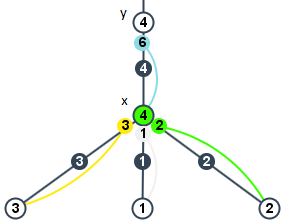
\includegraphics[width=\textwidth]{bilder/abb_paper_n-1knoten.png}
					\captionof{figure}{Der Wert der neuen Nachricht $\lambda_{y}$(blau) von Knoten x zu Knoten y beträgt 6, da $l_{2} + \omega(x) = 6$ (grün) größer ist als $l_{1} = 3$ (gelb).}
					\label{abb_n-1}
				\end{minipage}
				
				
			\item Der aktuelle Knoten x hat bereits von allen n zu ihm inzidenten Knoten eine Nachricht erhalten, selber jedoch noch nicht zu allen Knoten eine Nachricht gesendet. Diese Nachrichten müssen nun berechnet und versendet werden:\label{labelAufUnterfall}
			\\
				
				\begin{minipage}{0.50\textwidth} 
					
					Um eine Nachricht von x an einen Nachbarknoten y zu senden, der bis zu diesem Zeitpunkt noch keine Nachricht von x erhalten hat, nimmt man die 2 größten Nachrichten ($l_{1}$ und $l_{2}$), die bereits bei x angekommen sind. Dabei ist es wichtig, dass weder $l_{1}$ noch $l_{2}$ von y stammen. Die Nachricht von y wird bei dieser Nachrichtenberechnung ignoriert! Mit den beiden ermittelten Nachrichten $l_{1} \ge l_{2}$ sowie dem Knotengewicht $\omega(x)$ wird die Nachricht $\lambda_{y}$ an y wie folgt berechnet (Abbildung \ref{abb_n}):\\
					$\lambda_{y} = max\{l_{1},  l_{2} + \omega(x)\}$
					\\
					\\
					Diese Berechnung wird für jeden Nachbarknoten von x wiederholt, sodass jeder Nachbar eine Nachricht von x erhält. Nach diesem Schritt ist der Knoten x mit dem Algorithmus fertig, da er sowohl von jedem Nachbar eine Nachricht erhalten hat, als auch an jeden Nachbar eine Nachricht gesendet hat.
				\end{minipage}
				\hfill
				\begin{minipage}{0.35\textwidth}
					
					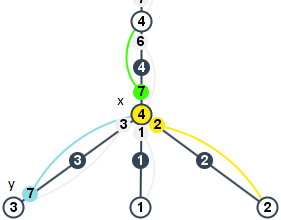
\includegraphics[width=\textwidth]{bilder/abb_paper_nknoten.png}
					\captionof{figure}{Die neue Nachricht $\lambda_{y}$ (blau) von Knoten x zu Knoten y hat den Wert 7, da $l_{1} = 7$ (grün) größer ist als $l_{2} + \omega(x) = 6$ (gelb).}
					\label{abb_n}
				\end{minipage}
			
		\end{enumerate}
		
	\item Fall:
		
		\begin{minipage}{0.55\textwidth} 
			Zu beginn des Algorithmus, oder wenn der Fall \ref{paperAlgoFall1} nicht mehr auftritt, sendet ein beliebiger Blattknoten seine Nachricht an den eigenen Nachbarn.\\
			
			Die zu sendende Nachricht $\lambda_{y}$ vom Blatt x an seinen Nachbarknoten y ist dabei nur das eigene Gewicht (Abbildung \ref{abb_leaf}):\\
			$\lambda_{y} = \omega(x)$
		\end{minipage}
		\hfill
		\begin{minipage}{0.35\textwidth}
						
			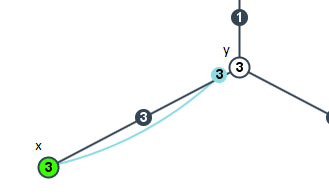
\includegraphics[width=\textwidth]{bilder/abb_blattknoten.png}
			\captionof{figure}{Das Knotengewicht des Blattknotens x (grün) bestimmt den Wert Nachricht $\lambda_{y} = 3$ (blau) zum Nachbarknoten y.}
			\label{abb_leaf}
		\end{minipage}
		
\end{enumerate}


%\subsubsection*{Berechnung der minimalen Agenten}

Sobald alle Knoten sowohl an alle Nachbarn eine Nachricht geschickt haben, als auch von allen Nachbarn eine Nachricht erhalten haben (jede Kante im gesamten Baum überträgt genau 2 Nachrichten), hat jeder Knoten alle Informationen die er gebraucht werden, um die minimale Anzahl an Agenten zu errechnen, die für diesen Knoten als Homebase benötigt werden.

\begin{mydef}
	Die minimale Anzahl an Agenten $\mu(x)$ ist die Agentenzahl, welche benötigt wird, um den gesamten Baum vom Knoten x aus zu dekontaminieren. Der Knoten x ist die Homebase, da von hier aus die Dekontaminierung beginnt.
\end{mydef}

Die minimale Agentenanzahl $\mu(x)$, die am Knoten x benötigt werden, wenn dieser als Homebase definiert wird, wird wie folgt berechnet:
\\
$\mu(x) = max\{l_{1},  l_{2} + \omega(x)\}$, wobei analog zu der Berechnung der Nachrichten gilt: $l_{1} \ge l_{2}$ sind die größten beiden angekommenen Nachrichten und $\omega(x)$ ist das Knotengewicht von x.
\\
\\
Nachdem alle Knoten ihr $\mu$ berechnet haben, wird ein Knoten mit minimalen $\mu$ ausgewählt. Dieser ist die neue Homebase, von dem aus $\mu$ viele Agenten den gesamten Baum dekontaminieren können, ohne die Monotonie-Eigenschaft zu verletzen (siehe oben).

\newpage

\subsection{Modifikationen am Algorithmus}\label{modifizierterAlgoChapter}


	\begin{wrapfigure}{l}{0.35\textwidth}
		\begin{center}
			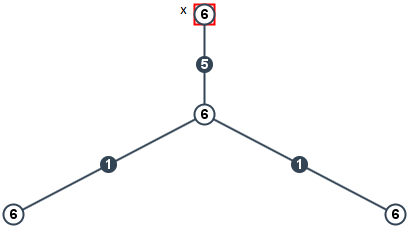
\includegraphics[width=0.35\textwidth]{bilder/abb_paper_problem.png}
		\end{center}
		\caption{Problem mit dem Algorithmus aus dem Paper. Der Knoten x sollte intuitiv mit 5 Agenten auskommen}
		\label{fig:negBeispielPaperAlgo}
	\end{wrapfigure}

Die Ergebnisse des im Paper beschriebene Algorithmus stimmt in einigen Fällen nicht mit der Intuition überein, die man bekommt wenn man einige Beispielbäume betrachtet (z.B. Abbildung \ref{fig:negBeispielPaperAlgo}). In dem  angegebenen Beispiel sollte der Knoten x mit 5 Agenten auskommen: Alle 5 Agenten gehen über die erste Kante zum mittleren Knoten. Von dort aus werden nur noch 2 Agenten benötigt: Einer hält Wache um die Monotonie zu gewährleisten und der zweite dekontaminiert ein Blatt. Zum Schluss wird das letzte Blatt von einem Agenten dekontaminiert und der Algorithmus ist fertig.
\\
Der Unterschied zwischen dem originalen Algorithmus und der Intuition ist folgender: Der originale Algorithmus plant im Beispiel für den mittleren Knoten 5 Wachen ein (das Knotengewicht ist 5), obwohl wir über die Kante mit Gewicht 5 gekommen sind, diese dadurch dekontaminiert ist, und wir sie nicht mehr bewachen müssen. Es werden dadurch mehr Agenten eingeplant, als wirklich benötigt werden.
\\
Da das Problem, wie erläutert, am Knotengewicht liegt, werde ich im folgenden eine Variante des Algorithmus beschreiben, die etwas anders mit dem Knotengewicht umgeht. Allerdings kommt es zu Fehlern, wenn man nur das Knotengewicht verändert, weshalb man zusätzliche Fälle in den Algorithmus einbauen muss, damit dieser sowohl richtig, als auch intuitiv sinnvoll funktioniert:
\\
\\
Im Gegensatz zum originalen Algorithmus wird im modifizierten Algorithmus nicht mehr das Knotengewicht in die direkte Berechnung der Nachricht miteinbezogen, sondern dient nur noch dazu, zu überprüfen, dass die berechnete Nachricht nicht zu klein ist.
\\
Dazu muss der Algorithmus in Kapitel \ref{paperAlgoChapter} Fall \ref{paperAlgoFall1} wie folgt abgeändert werden:

\subsubsection*{Modifizierte Berechnung der Nachricht:}

\begin{enumerate}[label=\alph*)]
	
	\item 
		Um eine Nachricht an einen Nachbarknoten y zu senden, der bis zu diesem Zeitpunkt noch keine Nachricht von x erhalten hat, nimmt man das Kantengewicht der zwei größten Kanten ($edge_{1}$ und $edge_{2}$) die inzident zu x sind, jedoch nicht zu y. Mit den beiden ermittelten Kantengewichten, für die gilt $edge_{1} \ge edge_{2}$ wird die Nachricht $\lambda_{y}$ an y wie auch in Abbildung \ref{modifiziert_a} gezeigt berechnet:\\
		$\lambda_{y} = edge_{1} + edge_{2}$.
		\\
		\\
		Vor der Bestimmung der zwei maximalen Kanten werden $edge_{1}$ und $edge_{2}$ auf 0 initialisiert, sodass die Berechnung auch klappt, falls es weniger als zwei Kanten gibt, auf die die Bedingung inzident zu x und nicht inzident zu y  zutrifft.
	
	\item
		Nachdem die neue Nachricht $\lambda_{y}$ nun berechnet wurde, müssen wir noch überprüfen, dass $\lambda_{y}$ nicht kleiner ist als das Knotengewicht $\omega(x)$. Ist dies der Fall bedeutet dass, dass das Kantengewicht der Kante, über die wir die Nachricht nach y schicken größer ist als die berechnete Nachricht. Da dies nicht sein darf, da wir sonst nicht genug Agenten haben würden, um über die Kante zu laufen, müssen wir die Nachricht die wir an y schicken entsprechend anpssen (Beispiel in Abbildung \ref{modifiziert_b}):
		
		\begin{algorithmic}
			\If {$\lambda_{y} \leq \omega(x)$}
			\State $\lambda_{y} \gets \omega(x)$
			\EndIf
		\end{algorithmic}
	
	\item
		Außerdem darf die berechnete Nachricht $\lambda_{y}$ nicht kleiner sein als die größte in x angekommene Nachricht $l_{1}$ (außer der Nachricht, die wir evt. schon von y erhalten haben). Ist die Nachricht $\lambda_{y}$ kleiner als $l_{1}$, würden wir nicht genug Agenten bekommen, um den Teilbaum, aus dem $l_{1}$ kommt zu dekontaminieren. Wir müssen $\lambda_{y}$ kontrollieren und evt. wie in Abbildung \ref{modifiziert_c} anpassen:
		
		\begin{algorithmic}
			\If {$\lambda_{y} \leq l_{1}$}
			\State $\lambda_{y} \gets l_{1}$
			\EndIf
		\end{algorithmic}
	
\end{enumerate}

\begin{figure}[h]
	\subfigure[Die Nachricht $\lambda_{y}$ (blau) von x zu y hat den Wert 5, da $edge_{1} $ und $edge_{2}$ (beide grün) die entscheidenden Kanten sind.
	\label{modifiziert_a}]{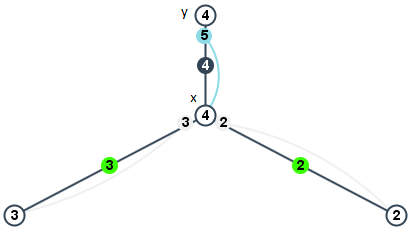
\includegraphics[width=0.32\textwidth]{bilder/abb_neu_max1max2.png}}
	\hfill
	\subfigure[Da das Knotengewicht durch die Kante zwischen x und y bestimmt wird (grün) und dieses größer ist als die Summe der beiden normalen Kanten $edge_{1}$ und $edge_{2}$ (gelb), bestimmt diese Kante den Wert der Nachricht $\lambda_{y} = 5$ (blau). \label{modifiziert_b}]{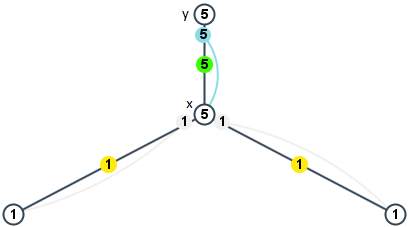
\includegraphics[width=0.32\textwidth]{bilder/abb_neu_edge.png}} 
	\hfill
	\subfigure[Die größte Nachricht (grün), die an x ankommt ist größer als die beiden Kanten $edge_{1}$ und $edge_{2}$ (gelb) und bestimmt dadurch den Nachrichtenwert $\lambda_{y} = 8$ (blau). \label{modifiziert_c}]{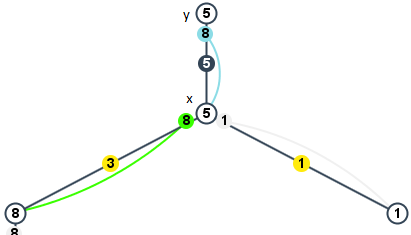
\includegraphics[width=0.32\textwidth]{bilder/abb_neu_msgData.png}}  
	
	\caption{Drei Fälle, die bei der Modifizierung des Algorithmus beachtet werden müssen, um alle Spezialfälle abzudecken.} 
	
	
	\begin{theorem}
		Die Modifikationen des Algorithmus ändern nichts an der linearen Laufzeit.
	\end{theorem}
	\begin{proof}
		Die Grundidee des Algorithmus bleibt erhalten. Jeder Knoten schickt zu all seinen Nachbarn je eine Nachricht. Die Anzahl der Nachrichten ändert sich durch die Modifikation nicht, sondern nur die Berechnung an sich.\\Die Berechnung kann in konstanter Zeit durchgeführt werden, das pro Knoten nur drei Schritte notwendig sind:
		\begin{enumerate}
			\item Berechnung der Nachricht durch einfache Addition
			\item Vergleich der Nachricht (und evt. Anpassen) mit dem Knotengewicht
			\item Vergleich der Nachricht (und evt. Anpassen) mit der maximalen Nachricht.
		\end{enumerate}
		Die lineare Zeit des als Grundlage verwendeten Algorithmus ist im erwähnten Paper bereits bewiesen worden.
	\end{proof}
\end{figure} 





	\section{Das Potential-Problem}\label{kap_pot}

Im Folgenden werden wir mich mit dem Hauptthema dieser Bachelorarbeit, dem Potential-Problem, beschäftigen.

\begin{mydef}\label{def_potential}
	Das Potential $k$ ist eine Art Kontostand, mit dem eine oder mehrere Kantengewichte reduziert werden können. Die Größe des Potentials gibt an, um wie viel die Gewichte insgesamt reduziert werden dürfen. 
\end{mydef}
Durch die Anwendung des Potentials soll sich die Anzahl der benötigten Agenten möglichst stark reduzieren, indem die Kante(n), die für die hohe Agentenzahl verantwortlich sind, reduziert werden.
\\
\\
Ich betrachte verschiedene Varianten des Potential-Problems und werde für jede Variante einen Algorithmus angeben und kurz Laufzeit und Korrektheit begründen.

\subsection{Spezialfall $k = 1$}\label{kap_pot=1}

Zunächst beschreiben wir das Potential-Problem $k = 1$, da dies die einfachste Variante ist. In dieser Variante darf auf genau einer beliebigen Kante das Kantengewicht um genau 1 reduziert werden. Allerdings muss das Gewicht der Kante nach der Reduzierung weiterhin $\omega \geq 1$ sein. Ziel ist es, das Potential so anzuwenden, dass die Anzahl der Agenten möglichst gut gesenkt wird.


\subsubsection{Algorithmus Idee}

Jeder Knoten berechnet im Algorithmus von \cite{cima_paper} die minimale Anzahl von Agenten (siehe Kapitel \ref{modifizierterAlgoChapter}), und es wird schnell klar, dass die Höhe der Agentenanzahl an jedem Knoten von bestimmten Kanten mit ihren Gewichten abhängen muss.
\\
\\
Die Idee, um das Potential-Problem für den Spezialfall $k = 1$ zu lösen, ist nun, die Abhängigkeiten zu speichern, welche Kanten die Agentenzahl in jedem Knoten beeinflussen. Dazu protokollieren wir im modifizierten Algorithmus (aus Kapitel \ref{modifizierterAlgoChapter}), wie jede berechnete Nachricht zustande kommt, also von welchen Kanten sie abhängt.
\\
\\ 
Wie im Algorithmus beschrieben, kann man sehen, dass eine Nachricht $\lambda_{y}$ aus drei verschiedenen Fällen entstehen kann:

\begin{enumerate}[label=\alph*)]
	
	\item aus den beiden größten Kanten $\lambda_{y} \gets edge_{1} + edge_{2}$ \label{entstehung_nachricht_max1+max2}
	
	\item aus der Kante, über welche die Nachricht gerade verschickt wird (diese entspricht dem Knotengewicht) $\lambda_{y} \gets \omega(x)$
	
	\item aus der größten angekommenen Nachricht $\lambda_{y} \gets l_{1}$

\end{enumerate}

Je nachdem, durch welchen Fall eine Nachricht $\lambda_{y}$ berechnet wird, kommen andere Kanten in Frage, die wir protokollieren müssen.
Allerdings gilt für alle Fälle, dass wir uns maximal zwei Kanten merken müssen, da wir ansonsten die minimale Agentenzahl nicht verringern können. Gibt es keine oder mehr als zwei Kanten, so merken wir uns nur die Information, dass das Potential an dieser Stelle nicht eingesetzt werden kann, um die Agentenzahl zu reduzieren (wir setzen eine "'flag"').

\begin{theorem}\label{theorem_max2kanten}
	Es müssen maximal zwei Kanten pro Nachricht protokolliert werden. Ansonsten kann das Potential nicht angewendet werden.
\end{theorem}

\begin{proof}
	Wir beweisen dieses Theorem, indem wir einen Widerspruch erzeugen. Wir nehmen an, es könnten mehr als zwei Kanten pro Nachricht protokolliert werden, o.B.d.A. seinen es drei Kanten. Dies würde bedeuten, dass wir durch Reduzierung einer dieser drei Kanten die Nachricht verkleinern könnten. Die Berechnung der Nachricht pro Fall hängt aber nur von maximal zwei Kanten ab (bei dem gerade beschriebenen Fall \ref{entstehung_nachricht_max1+max2} $\lambda_{y} \gets edge_{1} + edge_{2}$). Dies bedeutet, dass die drei Kanten aus zwei verschiedenen Fällen stammen müssen. Wenn also nun eine der drei Kanten reduziert wird, kann sich maximal nur ein Fall verkleinern, der andere bleibt unverändert. Da der Fall ausschlaggebend ist, der die größte Nachricht generiert, wird durch die Reduzierung der Kante die Nachricht nicht verändert, da der nicht veränderte Fall immer noch die alte Nachricht generiert. Da wir aber gesagt haben, dass alle drei Kanten die Nachricht reduzieren können, ist dies ein Widerspruch dazu, dass eine Nachricht von mehr als zwei Nachrichten abhängen kann.
\end{proof}

\subsubsection{Die Protokollierung in der Nachricht}

Im Folgenden werden wir bei allen drei möglichen Fällen beschreiben, welche Kanten unter welcher Bedingung protokolliert werden. Um protokollieren zu können, wird die Nachricht etwas erweitert. Sie enthält nun nicht mehr nur die Anzahl der Agenten, die für den Teilbaum benötigt werden, sondern auch die (bis zu) zwei protokollierten Kanten bzw. einen "flag", falls keine eindeutigen Kanten bestimmt werden konnten. Die Berechnung der Nachricht bleibt unverändert. Es wird nur zusätzlich folgende Protokollierung in den drei Fällen eingeführt: 

\begin{enumerate}[label=\alph*)]
	
	\item In diesem Fall wird die Nachricht aus den beiden größten Kanten berechnet ($\lambda_{y} \gets edge_{1} + edge_{2}$). Allerdings müssen wir kontrollieren, ob diese zwei Kanten eindeutig sind, oder ob es evtl. mehrere gleich große Kanten gibt. Ist die Wahl der Kanten nicht eindeutig, müssen wir dies bei der Protokollierung mit berücksichtigen:\\
	
		\begin{algorithmic}
			\If {$edge_{1} == edge_{3}$}
			\State \uline{protokolliere: "flag"}
			\LineComment{Es gibt (mindestens) drei gleich große Kanten. Selbst wenn man eine der drei Kanten reduziert, wird die Nachricht aus den anderen beiden Kanten berechnet und dadurch nicht verkleinert.}
			\ElsIf {$edge_{2} == edge_{3}$}
			\State \uline{protokolliere: $edge_{1}$}
			\LineComment{Die maximale Kante ist eindeutig, die zweit größte Kante nicht. Es macht also nur Sinn die größte Kante zu reduzieren.}
			\Else
			\State \uline{protokolliere: $edge_{1}$ und $edge_{2}$}
			\LineComment{Sowohl die größte, als auch die zweit größte Kante ist eindeutig. Wir können eine von den beiden reduzieren, um auch die Nachricht erfolgreich zu verkleinern.}
			\EndIf
		\end{algorithmic}
	
	\item Die Nachricht ist kleiner als das Knotengewicht: $\omega(x) > edge_{1}+edge_{2}$. Da aber $\omega(x)$ so definiert ist, dass es den Wert des größten Kantengewichts inzident zu $x$ hat, muss die Kante ausschlaggebend sein, über die die Nachricht verschickt wird. 
	\\
	Diese Kante $e = \{x, y\}$ zwischen $x$ und $y$ ist für den Nachrichtenwert also entscheidend und wird somit in der Nachricht protokolliert: \uline{Protokolliere: $e = \{x, y\}$}.
	
	\item In diesem Fall bestimmt die größte ankommende Nachricht $l_{1}$ die neu berechnete Nachricht. Da keine weitere Kante mehr Einfluss genommen hat, übernehmen wir die protokollierten Kanten (oder die "'flag"') aus $l_{1}$ für $\lambda_{y}$: \uline{Protokolliere: das gleiche wie $l_{1}$}
	
\end{enumerate}
Wichtig ist noch zu beachten, dass mehrere Fälle gleichzeitig auftreten können. Passiert dies, muss man einen weiteren Test durchführen, ob die verschiedenen Fälle unterschiedliche Kanten bzw. "'flag"' protokollieren würden.
\\
Würden die Fälle verschieden protokollieren, so protokolliere "'flag"', da es keine eindeutige(n) Kante(n) gibt, und somit das Potential an dieser Stelle nicht genutzt werden kann. Würden die verschiedenen Fälle exakt die gleiche(n) Kante(n) protokollieren, so wird diese Protokollierung für $\lambda_{y}$ übernommen.

\subsubsection{Protokollierung im Knoten}

Die Berechnung der $\mu$ an jedem Knoten funktioniert analog zur Nachrichtenberechnung. Auch in den Knoten wird gespeichert, von welchen Kanten der Wert abhängt. Dies ist entweder $edge_{1}$ und $edge_{2}$, oder die Kanten, die in $l_{1}$ protokolliert sind.
\\
\\
Nachdem jeder Knoten $x$ den Wert $\mu(x)$ berechnet hat und die Kanten gespeichert hat, von denen dieser Wert abhängt, geht der Algorithmus durch alle Knoten durch und speichert von jedem Knoten $i$, für den gilt $\mu(i) = \mu(h)$, wobei $h$ die Homebase ist, von welchen Kanten dieser Knoten $i$ abhängt, in einer Liste $L$. \\
Das Potential wird auf eine dieser in $L$ gespeicherten Kanten angewendet, um die Anzahl der Agenten zu minimieren. Falls das Potential $k = 1$ nicht angewendet werden kann, so ist $L$ leer.

\subsubsection{Laufzeit und Korrektheit}


	\begin{theorem}
		Die Protokollierung, und somit die Berechnung der Kante, auf die das Potential $k=1$ angewendet werden sollte, ist in linearer Laufzeit möglich.
	\end{theorem}
	\begin{proof}
		Um die Laufzeit abzuschätzen, reicht es, die Berechnung der Nachrichten zu betrachten, da nur diese für den Algorithmus verändert wurde. Die Anzahl der zu berechnenden Nachrichten weicht nicht von der benötigten Anzahl des Algorithmus in Kapitel \ref{modifizierterAlgoChapter} ab. Außerdem kann die Protokollierung für jede Kante in konstanter Zeit durchgeführt werden. Für jede Nachrichtenberechnung muss nur eine einfache Fallunterscheidung durchgeführt werden, um zu ermitteln, welche Kante in der aktuellen Nachricht protokolliert werden muss. Da es $O(n)$ viele Nachrichten gibt, die alle in $O(1)$ berechnet werden können, bleibt die Laufzeit, wie in Theorem \ref{thm_laufzeit_modifikation}, linear.
	\end{proof}
	
	\begin{theorem}
		Bei jeder Nachricht werden die richtigen Kanten protokolliert. Dadurch erhält jeder Knoten $x$ die korrekte Information, von welchen Kanten das $\mu(x)$ abhängt. 
	\end{theorem}
	\begin{proof}
		Die Korrektheit folgt aus der Konstruktion: Es gibt nur die beschriebenen drei Fälle, aus welchen Kanten eine Nachricht bestehen kann. Die Kanten, aus denen die entsprechende Nachricht berechnet wird, werden mit in der Nachricht protokolliert.\\
		Auch die "'flag"' wird richtig gesetzt. Wenn es keine oder mehr als zwei Kanten gibt, die protokolliert werden müssten, kann man das Potential an dieser Stelle nicht einsetzen, und die "'flag"' wird in der Nachricht protokolliert. Dies folgt direkt aus Lemma \ref{theorem_max2kanten}.
		\\
		\\
		Die Berechnung vom $\mu$ an jedem Knoten erfolgt analog zur Berechnung der Nachrichten. Jeder Knoten kann speichern, von welchen Kanten sein $\mu$ abhängt: Entweder von $edge_{1}$ und $edge_{2}$, oder von einer der angekommenen Nachrichten, die auch jeweils die Information gespeichert haben, von welchen Kanten sie abhängen.\\
		Auch die Liste $L$ ist korrekt. Da das Potential in diesem Spezialfall nur 1 beträgt, kann sich die Anzahl der Agenten auch nur um eins reduzieren. Daher kommen nur Knoten in Frage, die bereits nur das Minimum an Agenten benötigen, also so viele wie auch die Homebase. Ein anderer Knoten kann seinen Wert im besten Fall nur auf diesen Wert reduzieren. Daher geht der Algorithmus alle Knoten durch, die das Minimum an Agenten haben und schaut, ob (mindestens) einer von diesen Knoten reduziert werden kann, bzw. eine Kante gespeichert hat, um diesen zu reduzieren. Alle möglichen Kanten befinden sich daher in der Liste $L$, und falls diese leer ist, kann das Potential nicht angewendet werden.
		
	\end{proof}


\subsection{Potential auf einer Kante mit $k \geq 1$}\label{kap_pot>=1}


Um das Potential-Problem etwas zu erweitern, betrachten wir im folgenden Abschnitt Potentiale $k \geq 1$, allerdings mit der Einschränkung, dass man das gesamte Potential $k$ nur auf einer Kante einsetzen darf.

\begin{theorem}
	Man kann trotz beliebig großem Potential nicht garantieren, dass sich die minimale Anzahl an benötigten Agenten reduziert, wenn das Potential nur auf einer Kante eingesetzt werden darf.
\end{theorem}

\begin{proof}
	Wir nehmen an, es sei mit beliebig großem Potential immer möglich, die Anzahl der benötigten Agenten zu reduzieren.
	\\
	\\	
	Da das Potential $k$ beliebig groß ist, kann man die Kante, auf welche man das Potential anwenden möchte, auf Kantengewicht 1 setzen. Dadurch kann man garantieren, dass das größtmögliche Potential eingesetzt worden ist, da jede Kante immer ein Gewicht $\omega \geq 1$ haben muss. Trotzdem ist es nicht möglich bei folgendem Baum die Anzahl der Agenten zu reduzieren (siehe Abbildung \ref{abb_gegenbeispielMaxPotential}). Da dieser Baum absolut symmetrisch ist, spielt es keine Rolle, auf welche der vier Kanten das Potential angewendet wird und das Kantengewicht auf 1 gesetzt wird.
	
	\begin{figure}[hbt]
		\subfigure[alle Kanten haben Gewicht 4. Alle Knoten benötigen mindestens 8 Agenten.]{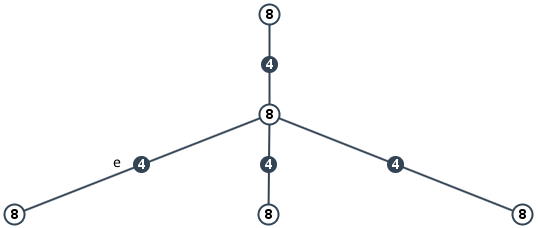
\includegraphics[width=0.65\textwidth]{bilder/abb1.png}} 
		%		\hfill
		
		\subfigure[eine Kante wurde auf Gewicht 1 geduziert, alle anderen haben weiterhin Gewicht 4. Alle Knoten benötigen trotzdem mindestens 8 Agenten.]{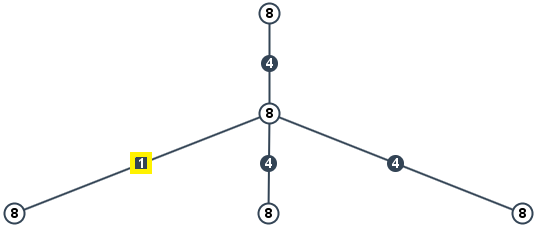
\includegraphics[width=0.65\textwidth]{bilder/abb2.png}} 
		\captionsetup{width=0.9\textwidth}
		\caption{Beispiel, dass Verringerung auf einer Kante nicht zu einer Verringerung der notwendigen Agenten führen muss} 
		\label{abb_gegenbeispielMaxPotential}
	\end{figure} 
	
	Da das Potential in diesem Gegenbeispiel nicht angewendet werden kann, ist dies ein Widerspruch zur Annahme, dass man die Agentenanzahl auf einem beliebigen Baum mit beliebig großem Potential immer reduzieren kann.
\end{proof}

Trotzdem ist es möglich, einen Algorithmus anzugeben, der die Kante auswählt, welche die Agentenanzahl am meisten minimiert, falls es eine solche Kante gibt.


\subsubsection{Algorithmus Idee}

	Auch um dieses Problem zu lösen, muss die in Kaptiel \ref{modifizierterAlgoChapter} benutze Nachricht angepasst werden. Die Idee dieses Algorithmus ist es - ähnlich wie beim Spezialfall $k = 1$ -  Protokoll zu führen. Damit lässt sich im Anschluss bestimmen, welche Kante am sinnvollsten reduziert werden muss.\\
	Jeder Knoten $x$ soll am Ende des Algorithmus folgende Informationen haben:
	\begin{itemize}
		\item $\mu(x)$: die normale Agentenanzahl (wird wie in Kapitel \ref{modifizierterAlgoChapter} ganz normal berechnet).
		\item $\hat{\mu}(x)$: die benötigte Anzahl an Agenten, die durch für diesen Knoten optimale Anwendung des Potentials erreicht werden kann.
		\item $e_{1}, e_{2}$: die Kanten, auf die das Potential angewendet werden muss, um $\hat{\mu}(x)$ zu erreichen.
	\end{itemize}
	Hat jeder Knoten am Ende des Algorithmus diese Informationen, kann man mit einem Durchlauf durch alle Knoten das Minimum aller $\hat{\mu}$ ermitteln. Dies ist dann die kleinste Anzahl an Agenten, die man durch das Potential erreichen kann. Da außerdem gespeichert ist, welche Kanten dafür reduziert werden müssen, kann man auf eine dieser Kanten das Potential anwenden, um die Agentenzahl entsprechend zu reduzieren. Wie in Theorem \ref{theorem_max2kanten} argumentiert, kommen immer nur maximal zwei Kanten pro Knoten in Frage.
	
	\subsubsection{Berechnung der Nachricht}
	
	Um diese Informationen zu generieren, müssen die Nachrichten erweitert werden.
	Diese enthalten nun folgende Parameter:
	\begin{itemize}
		\item $\alpha$: die normal berechnete Nachricht (siehe Kapitel \ref{modifizierterAlgoChapter})
		\item $\beta$: modifizierte Nachricht, die durch das Potential am stärksten reduzierte Nachricht
		\item $e_{1} / e_{2}$: die Kanten, auf die das Potential angewendet worden ist
	\end{itemize}
	Es bleibt noch zu klären, wie die modifizierte Nachricht $\beta$ und die Kanten $e_{1}$ und $e_{2}$ berechnet werden:\\
	Bei jeder Berechnung einer neuen Nachricht kommen nur bis zu vier Möglichkeiten in Frage, wie das Potential angewendet werden kann, um die richtige modifizierte Nachricht zu generieren. Diese vier Möglichkeiten sind: $edge_{1}$, $edge_{2}$, $edge_{xy}$ (also die Kante, über die die Nachricht geschickt wird) und die Protokollierung von $l_{1}$ als größte Nachricht. Um nun herauszufinden, wie das Potential an dieser Stelle am effektivsten angewendet werden muss, werden alle vier Möglichkeiten nacheinander ausprobiert und dann entschieden, wo das Potential die größte Reduzierung zur Folge hatte. Der Fall mit dem größten Effekt wird in der neuen Nachricht gespeichert.
	\\
	\\
	Wir gehen alle Fälle durch, um die modifizierte Nachricht $\beta$ von Knoten $x$ nach $y$ zu berechnen:
	\begin{enumerate}
		\item berechnet $\beta$, indem das Potential auf die Kante zwischen x und y angewendet wird ($edge_{xy} - potential$).
		\item berechnet $\beta$, indem das Potential auf die größte Kante $edge_{1}$ angewendet wird ($edge_{1} - potential$) .
		\item berechnet $\beta$, indem das Potential auf die zweitgrößte Kante $edge_{2}$ angewendet wird ($edge_{2} - potential$).
		\item berechnet $\beta$, indem aus $l_{1}$ nicht die normale Nachricht $\alpha$, sondern die modifizierte Nachricht $\beta$ verwendet wird.
	\end{enumerate}
	Der kleinste $\beta$-Wert aus diesen vier Fällen ist unsere modifizierte Nachricht $\beta$. Die Kanten, auf die das Potential angewendet wurde, wird als 3. Parameter $e_{1} / e_{2}$ in der Nachricht mit verschickt.\\
	Treten mehrere Fälle auf, die zu einen identischen $\beta$-Wert führen, so muss ein weiterer Test durchgeführt werden, ob es sich um die gleichen Kanten $e_{1} / e_{2}$ handelt. 
	\\
	\\
	Zu beachten ist noch, dass jede Kante zu jeder Zeit ein Kantengewicht $\omega \geq 1$ haben muss. Also wenn z.B. $edge_{1} - potential$ einen Wert $\beta < 1$ liefert, muss dieser Wert auf 1 gesetzt werden.
	\\
	\\
	Die Vorgehensweise ändert sich im Gegensatz zu dem Algorithmus aus Kapitel \ref{modifizierterAlgoChapter} nicht. Auch das $\alpha$ der Nachricht wird, wie im Algorithmus beschrieben, berechnet.
	
	
	\subsubsection{Berechnung der minimalen Agenten}
	
	Um nun das $\hat{\mu}$ jedes Knotens zu berechnen, gehen wir analog zur Berechnung der Nachricht vor. Der einzige Unterschied ist, dass es einen Fall weniger gibt: 
	\begin{enumerate}
		\item berechnet $\hat{\mu}$, indem das Potential auf die größte Kante $edge_{1}$ angewendet wird ($edge_{1} - potential$) .
		\item berechnet $\hat{\mu}$, indem das Potential auf die zweitgrößte Kante $edge_{2}$ angewendet wird ($edge_{2} - potential$).
		\item berechnet $\hat{\mu}$, indem aus $l_{1}$ nicht die normale Nachricht $\alpha$, sondern die modifizierte Nachricht $\beta$ verwendet wird.
	\end{enumerate}
	Da wir keine Nachricht mehr verschicken müssen, sondern nur noch das $\hat{\mu}$ ausrechnen wollen, fällt der Fall, in dem wir auch die Kante $edge_{xy}$ reduzieren müssen, weg.\\
	Nachdem wir für jeden Knoten die drei Parameter ausgerechnet haben, wissen wir für jeden Knoten, wie viele Agenten wir brauchen, wenn wir das Potential nicht anwenden ($\mu$); wie viele Agenten wir benötigen, wenn wir das Potential anwenden $\hat{\mu}$; und auf welche Kanten wir das Potential anwenden müssen, um diese Verbesserung zu erreichen (die Kanten, die wir zur Berechnung von $\hat{\mu}$ reduziert haben).\\
	Durch einen linearen Durchlauf durch alle Knoten können wir nun das Minimum aller $\hat{\mu}$ berechnen und die dazugehörige(n) Kante(n) auswählen, auf die das Potential sinnvoll angewendet werden kann.
	\\
	\\
	Analog zur Nachrichtenberechnung muss jede Kante zu jedem Zeitpunkt der Berechnung ein Kantengewicht $\omega \geq 1$ haben muss. 
	
	
	\subsubsection{Laufzeit und Korrektheit}
	
	\begin{theorem}
		Die Berechnung aller Nachrichten und die Bestimmung der Kante, auf die das Potential angewendet werden sollte, ist in linearer Laufzeit möglich.
	\end{theorem}
	\begin{proof}
		Analog zu Theorem \ref{thm_laufzeit_modifikation} wird die Grundidee des Algorithmus nicht verändert. Jeder Knoten schickt zu all seinen Nachbarn je eine Nachricht. Die Anzahl der Nachrichten ändert sich durch die Modifikation nicht, sondern nur die Berechnung an sich.\\Die Berechnung der Nachricht kann auch hier in konstanter Zeit durchgeführt werden, da pro Nachricht nur maximal vier konstante Fälle berechnet werden müssen, und aus diesen das Minimum bestimmt werden muss.\\
		Auch die Berechnung der minimalen Agenten ist für jeden Knoten in konstanter Zeit möglich, wodurch der ganze Algorithmus eine Laufzeit von $O(n)$ hat.
	\end{proof}
	
	
	Um nun die Korrektheit des Algorithmus zu zeigen, muss man garantieren, dass jeder Knoten alle ausgehenden Nachrichten richtig berechnet. Wie beschrieben, enthält jede Nachricht drei Teilinformationen: $\alpha$, die normal berechnete Nachricht; $\beta$, die Nachricht, die man erhält, wenn man im aktuellen Teilbaum das Potential optimal anwendet; und $e_1/e_2$, die zwei Kanten, auf die das Potential angewendet werden muss, um die optimale Nachricht $\beta$ zu erhalten.
	\\
	\\
	Für die Korrektheit dieses Algorithmus ist nur $\beta$ interessant, da $\alpha$ die identische Nachricht aus Kapitel \ref{modifizierterAlgoChapter} ist, und wir die Kanten $e_1/e_2$ einfach aktualisieren können, wenn wir $\beta$ verändern. Daher können wir aus folgender Invariante schließen, dass der Algorithmus das Potential bis zum aktuellen Zeitpunkt richtig berechnet hat:
	
	\begin{theorem}
		Jeder Knoten im Baum berechnet korrekt, ob, und wenn ja, wo im aktuellen Teilbaum das gegebene Potential am effektivsten angewendet werden kann. Außerdem wird berechnet, wie groß die benötigte Agentenzahl nach Anwenden des Potentials für diesen Teilbaum ist.
	\end{theorem}
	\begin{proof}
		Um für die Korrektheit dieser Aussage zu argumentieren, muss man sich zwei Arten von Knoten anschauen: Blattknoten und innere Knoten im Baum.\\
		\\
		Zuerst betrachten wir die Blattknoten:\\
		Zu jedem Blatt führt genau eine Kante. Daher kann das Potential nur auf dieser einen Kante angewendet werden. Wenn die Nachricht nun von diesem Knoten berechnet wird, muss bei der Berechnung nur überprüft werden, ob sich die Nachricht verringert, wenn das Kantengewicht um das Potential reduziert wird. Dies ist immer der Fall, wenn das Kantengewicht $\omega > 1$ ist, da dadurch die Kante reduziert werden kann und man daher für diesen Teilbaum weniger Agenten benötigt.
		\\
		\\
		Betrachten wir nun einen beliebigen Knoten $x$ innerhalb des Baumes:\\
		Wir gehen davon aus, dass bis zu diesem Zeitpunkt alle Nachrichten korrekt berechnet wurden. Dann muss der Knoten $x$ aus allen seinen angekommenen Nachrichten die neue Nachricht berechnen.\\
		Der Knoten $x$ hat die Information, wie viele Agenten die einzelnen Teilbäume brauchen, wenn das Potential nicht angewendet wird, dies ist die normale Nachricht $\alpha$, und, wie viele Agenten die einzelnen Teilbäume benötigen, wenn das Potential in diesen angewendet wurde (dies ist der $\beta$-Wert der einzelnen Nachrichten). Außerdem kennt der Knoten $x$ all seine inzidenten Kanten.\\
		Das einzige, was wir jetzt noch garantieren müssen ist, dass der Knoten $x$ alle Informationen aus den einzelnen Teilbäumen und aus seinen inzidenten Kanten richtig zusammensetzt, und somit eine Nachricht an einen Knoten $y$ berechnet, die für den gesamten Teilbaum gilt.\\
		\\
		Es sind nur drei Kanten bei der Berechnung interessant: Die Kante, über die die Nachricht von $x$ nach $y$ geschickt wird, sowie die zwei größten Kanten $edge_1$ und $edge_2$, inzident zu $x$. Wenn eine andere Kante in diesem Teilbaum besser geeignet ist für das Potential, wurde sie schon in einer der Nachrichten an $x$ gespeichert. 
		\\
		\\
		Der Knoten $x$ muss daher nur testen, ob sich der $\beta$-Wert verbessert, wenn das Potential auf einer der drei Kanten angewendet wird, oder wenn wir von $l_{1}$ (also der größten angekommenen Nachricht) den $\beta$-Wert benutzen. Die Variante mit dem größten Einfluss ist der Wert für die neue Nachricht, und die entsprechende(n) Kante(n) werden in $e_1/e_2$ protokolliert.
		\\
		\\
		Die Berechnung von allen $\mu$-Werten erfolgt analog zu der Nachrichtenberechnung, sodass jeder Knoten die drei Parameter $\alpha$, $\beta$ und $e_1/e_2$ berechnet. \\
		Mit einem Durchlauf durch alle Knoten kann die größte Auswirkung des Potentials gefunden werden, sowie die zugehörigen Kanten, auf die das Potential angewendet werden kann.
		\\
		\\
		Falls es keine Möglichkeit gibt, das Potential anzuwenden, so gilt $\min \beta = \min \alpha$. Dies ist der Fall, wenn sich die minimale Anzahl an Agenten unabhängig von der Potentialanwendung nicht verändert.
	\end{proof}
	
	

\subsection{Potential verteilen mit $k > 1$}

Die nächste Erweiterung des Potentialproblems ist es, Potentiale $k > 1$ zu betrachten, bei denen man das Potential auf verschiedene Kanten verteilen kann.\\
In Abbildung \ref{abb_gegenbeispielMaxPotential} haben wir bereits ein Beispiel gesehen, in dem es tatsächlich nötig sein kann, das Potential auf verschiedene Kanten zu verteilen. Dieses Beispiel wollen wir im folgenden etwas erweitern und erläutern:

\begin{theorem}
	Es gibt Bäume, bei denen man das Potential auf linear viele Kanten verteilen muss.
\end{theorem}	
\begin{proof}
	Um dieses Theorem zu Beweisen, reicht es aus, ein Beispiel anzugeben, bei dem das Potential tatsächlich auf linear viele Kanten verteilt werden muss. Solch ein Beispiel kann man in Abbildung \ref{abb_bsp_potverteilen} finden. Der Baum besteht aus einem Wurzelknoten, der $n$ viele Kindknoten hat. Alle $n$ Kanten haben das gleiche Kantengewicht $\omega = 5$.
	
		\begin{figure}[htb]
			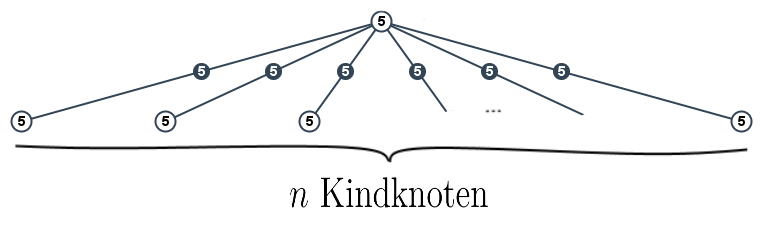
\includegraphics[width=0.65\textwidth]{bilder/abb_bsp_potverteilen.png} 
			\captionsetup{width=0.65\textwidth}
			\caption{Die Mindestanzahl an benötigten Kanten kann bei der Potentialverteilung kann eine Komplexität linear zur Knotenanzahl haben.}
			\label{abb_bsp_potverteilen}
		\end{figure}
		
	Um nun bei diesem Baum durch ein Potential $k$ die Agentenzahl verringern zu können, muss $k$ auf $n-2$ vielen Kanten angewendet werden, wobei $n$ die Anzahl der Kindknoten ist. Daraus folgt direkt, dass $k$ mindestens $n-2$ groß sein muss, damit wir das Potential überhaupt auf den Baum aus unserem Beispiel anwenden können. Bei einem geringeren Potential kann man keine Verbesserung erzielen.
	\\
	\\
	Bleibt noch zu klären, warum das Potential auf $n-2$ Kanten angewendet werden muss:
	\\
	Wie in Kapitel \ref{modifizierterAlgoChapter} beschrieben, kann eine Nachricht $\lambda_{x}$ aus drei Fällen bestehen. 
	\begin{enumerate}[label=\alph*)]
		\item aus den zwei größten Nachrichten: $\lambda_{x} = edge_{1} + edge_{2}$.
		\item aus der Kante, über welche die Nachricht geschickt wird: $\lambda_{x} = edge_{xy}$.
		\item aus der größten Nachricht: $\lambda_{x} = l_{1}$.
	\end{enumerate}	
	Allerdings ist nur der Fall $\lambda_{x} = edge_{1} + edge_{2}$ interessant, da sowohl die Kante $edge_{xy}$ eindeutig ist, als auch die größte angekommene Nachricht.
	\\
	\\
	Wenn man nun eine einzige, beliebige Kante reduziert, wird diese Reduzierung keinen Effekt haben, da diese Kante in der Berechnung $\lambda_{x} = edge_{1} + edge_{2}$ durch eine andere, gleich große Kante, ersetzt wird. Um also das Potential anwenden zu können, sodass tatsächlich die Agentenzahl an einem Knoten $x$ reduziert wird, muss man so lange eine Kante $e$ reduzieren, für die gilt: $\omega(e) = \max_{i} \omega(i)$ für alle zu $y$ inzidenten Kanten $i$, bis gilt $edge_{1} > edge_{2} \geq \dots \geq edge_{deg(y)-1}$
	\\
	Sobald diese Bedingung gilt, können die durch das Potential reduzierten Kanten nicht mehr ausgetauscht werden, da es keine Kante mehr gibt, die groß genug wäre. Die Berechnung $\lambda_{x} = edge_{1} + edge_{2}$ ist daher eindeutig und Der Knoten $x$ bekommt eine reduzierte Nachricht und somit eine reduzierte Knotenanzahl.
	\\
	Dafür muss man genau $n-2$ Kanten reduzieren, da man in dem Beispiel alle Kanten reduzieren muss, außer die Kante $e = {xy}$, über die die Nachricht geschickt wird und die Kante $edge{1}$. Alle $n$ Kanten, abzüglich dieser beiden Kanten ergibt $n-2$ Kanten.
	\\
	\\
	Die Idee dieses Beweises lässt sich auch aus Theorem \ref{theorem_max2kanten} herleiten, bei welchem wir eine ähnliche Eigenschaft ausgenutzt haben.
	
\end{proof}


.........................Bei den Potentialproblemen $k = 1$ (Kapitel \ref{kap_pot=1})und $k \geq 1$ auf einer Kante (Kapitel \ref{kap_pot>=1}) war es relativ einfach zu testen, auf welche Kante das Potential angewendet werden muss, um einen möglichst großen Effekt zu bekommen. Bei jeder Nachrichtenberechnung musste man nur konstant viele Kanten testen und es war daher möglich einen Algorithmus zu entwerfen, der ohne Laufzeitverschlechterung die jeweilige Kante bestimmen konnte.
\\
\\
.........................Wenn man das Potential aber auf verschiedene Kanten verteilen möchte, ist dies nicht mehr so leicht möglich. Es gibt nicht mehr nur konstant viele Kanten, die man pro Nachrichtenberechnung kontrollieren muss, sondern es kann passieren, dass man quadratisch viele Kanten in den Nachrichten speichern muss:\\
Wenn man das Beispiel aus Abbildung \ref{abb_bsp_potverteilen} erweitert (siehe Abbildung \ref{abb_bsp_potverteilen_quadratisch}), sieht man, dass............
	\begin{figure}[htb]
		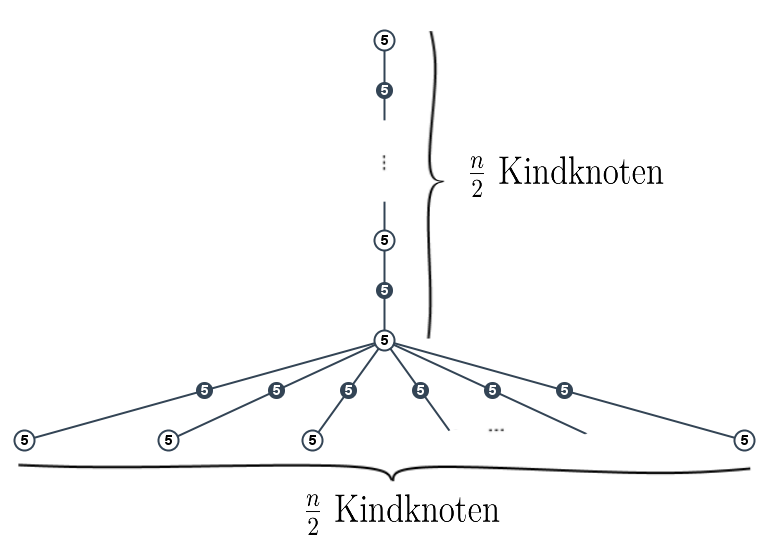
\includegraphics[width=0.65\textwidth]{bilder/abb_bsp_potverteilen_quadratisch.png} 
		\captionsetup{width=0.65\textwidth}
		\caption{Die Mindestanzahl an benötigten Kanten kann bei der Potentialverteilung kann eine Komplexität linear zur Knotenanzahl haben.}
		\label{abb_bsp_potverteilen_quadratisch}
	\end{figure}

	
	\section{Implementierung}\label{kap_implementierung}

Im Rahmen einer Projektarbeit im Wintersemester 2014/15 haben wir den in \cite{cima_paper} beschriebenen Algorithmus in einem Java-Applet implementiert. Ziel war es, den Algorithmus visuell darzustellen und ihn anhand des Applets in einem kurzen Vortrag vorzustellen.
\\
\\
Als Bestandteil dieser Bachelorarbeit haben wir das Applet mit der in Kapitel \ref{modifizierterAlgoChapter} beschriebenen Modifikation erweitert und die beiden Algorithmen in Kapitel \ref{kap_pot} entwickelt und ebenfalls in das Applet integriert.


\subsection{Benutzung des Applets}

Im Folgenden werden wir kurz beschreiben, wie das Applet benutzt werden kann:

\subsubsection*{Den Baum erstellen und ändern}

Man kann einen Baum (bzw. einen Baumknoten) erstellen, indem man mit einem Linksklick in das leere Applet klickt. Sofort erscheint ein Wurzelknoten.\\
Mit einem Linksklick auf einen Knoten fügt man ihm einen Kindknoten hinzu. Mit einem Rechtsklick auf einen Knoten wird dieser zusammen mit dem gesamten Teilbaum gelöscht.\\
Die Kantengewichte lassen sich ebenfalls mit einem Klick verändern. Ein Linksklick erhöht das entsprechende Kantengewicht um 1, ein Rechtsklick reduziert das Kantengewicht um 1. Allerdings können die Kantengewichte nicht kleiner als 1 werden.


\subsubsection*{Verwendung des Applets}

Nachdem man einen Baum erstellt hat, gibt es mehrere Funktionen, die man auswählen kann:\\

\begin{itemize}
	\item Man kann die Nachrichtenberechnung sowohl von dem ursprünglichen Algorithmus (Kapitel \ref{kap_algorithmus}), als auch von der Modifikation (Kapitel \ref{modifizierterAlgoChapter}) animieren lassen oder sofort das Ergebnis anzeigen. Bei der Animation wird immer angezeigt, wie jede einzelne Nachricht zustande kommt. Dies wird in Kurzform als Text und durch Färbung der einzelnen Elemente des Baumes verdeutlicht. Nachdem alle Nachrichten verschickt wurden, berechnet jeder Knoten, wie viele Agenten benötigt werden, um den gesamten Baum von diesen Knoten aus zu dekontaminieren. Dieser Wert wird am Ende in jedem Knoten angezeigt. Nach Abschluss des Algorithmus wird einer der Knoten mit minimaler Agentenzahl ausgewählt und als Homebase markiert.
	
	\item Alternativ zur Nachrichtenberechnung kann man sich die beiden Algorithmen aus Kapitel \ref{kap_pot} visuell darstellen lassen. Dazu werden ebenfalls die Nachrichten einzeln animiert (oder das Ergebnis sofort angezeigt), allerdings zeigen die Informationen (Text und Einfärbung), wie in jedem einzelnen Schritt die erweiterte Nachricht berechnet wird, die in dem jeweiligen Algorithmus benutzt wird. Man muss beachten, dass die Potentialberechnung nur mit der modifizierten Variante des Algorithmus ausführbar ist. Am Ende dieses Algorithmus wird angezeigt, wie viele Agenten jeder Knoten zu Dekontamination benötigt, welcher Knoten die Homebase ist, und, falls möglich, welche Kante reduziert werden sollte, um die Agentenzahl möglichst weit zu reduzieren.
	
	\item Außerdem lässt sich im Applet animieren, wie nach erfolgreicher Nachrichtenberechnung die Dekontamination des Baumes funktioniert. Die Strategie der Agenten ist dabei monoton. Dies bedeutet, dass jeder Knoten, der schon einmal dekontaminiert wurde, nicht mehr kontaminiert werden kann, da an den entsprechenden Stellen im Baum Wachen aufgestellt werden. Sind alle Knoten dekontaminiert, ist der Algorithmus abgeschlossen.
\end{itemize}

Alle Animationen können entweder als Ganzes abgespielt oder in einer Step-by-step-Animation in Teilen durchgeführt werden. \\
Alle Optionen, die im Applet verfügbar sind, werden eingeblendet. Alle in dem Moment nicht verfügbaren Optionen werden ausgeblendet, um eine bessere Übersicht zu gewährleisten.


\subsection{Beispiel aus dem Applet}

hier ist ein ganz tolles Beispiel....
	
	\section{Fazit}
Fazit...
	
	\newpage

%	\defaultsectionstyle
	\renewcommand{\refname}{Literaturquellen}
	
	\begin{thebibliography}{99}
		
		
		\bibitem[Ba02]{cima_paper} \textsc{L. Barrière, P. Flocchini, P. Fraigniaud, N. Santoro} (2002): Capture of an Intruder by Mobile Agents. (SPAA'02) Winnipeg, Manitoba, Canada.

		\bibitem[Fl08]{tdti_paper} \textsc{P. Flocchini, B. Mans, N. Santoro} (2008): Tree Decontamination with Temporary Immunity. (ISAAC'08) Gold Coast, Australia.
		
		\bibitem[Me88]{complexity_paper} \textsc{N. Megiddo, S. Hakimi, M. Garey, D. Johnson, C. Papadimitriou} (1988): The Complexity of Searching a Graph. Journal of the ACM, Vol. 35, No 1, 1988.
		
		\bibitem[Fi09]{firefighterproblem_paper} \textsc{S. Finbow, G. MacGillivray} (2009): The Firefighter Problem: A survey of results, directions and questions.
		AUSTRALASIAN JOURNAL OF COMBINATORICS Vol. 43 (2009), Pages 57–77
		
		\bibitem[Pa76]{graph_paper_76} \textsc{T. Parson} (1976): Pursuit-evasion problem in a graph. Theory and Applications of Graphs, Lecture Notes in Mathematics, Springer-Verlag, 426-441.
		
		\bibitem[Kl14]{klein_paper} \textsc{R. Klein, E. Langetepe, C.  Levcopoulos} (2014): A Fire Fighter's Problem. arXiv:1412.6065
		
		\bibitem[Neu96]{grid_paper_96} \textsc{N. Neufeld} (1996): A pursuit-evasion problem on a grid. Information Processing Letters, Vol. 58, No 1, 1996.
		
		\bibitem[Su92]{polygon_paper} \textsc{I. Suzuki, M. Yamashita} (1992): Searching for a mobile intruder in a polygonal region. SIAM Journal on Computing, Vol. 21, No 5.


		
	\end{thebibliography} 
	
	
\end{document}
